%!TeX program = xelatex
\documentclass[12pt,hyperref,a4paper,UTF8]{ctexart}
\usepackage{compiler_versions_recognition}
\usepackage{inputenc}
\usepackage[british,UKenglish]{babel}
\usepackage{amsmath}
\usepackage{algorithm}%算法
\usepackage{algorithmic}%算法
\usepackage{subfiles}%分文件编写章节
\usepackage{booktabs}
\usepackage{titlesec}
\usepackage{color}
\usepackage{graphicx}
\usepackage{subfigure}%子图
\usepackage{subcaption}%子图
\usepackage{fancyref}
\usepackage{hyperref}%超链接
\usepackage{float}%浮动图片
\usepackage{scrextend}
\usepackage{setspace}
\usepackage{xargs}
\usepackage{multicol}
\usepackage{nameref}
\usepackage{longtable}
\usepackage{sectsty}
\usepackage{booktabs}
\usepackage{longtable}
\usepackage{multicol}
\usepackage{multirow}
\usepackage{appendix}
\usepackage{listings}

\newcommand\tab[1][1cm]{\hspace*{#1}}
\hypersetup{colorlinks=true, linkcolor=blue}
\interfootnotelinepenalty=10000
% -------------------------允许算法跨页-------------
\makeatletter
\newenvironment{breakablealgorithm}
  {% \begin{breakablealgorithm}
   \begin{center}
     \refstepcounter{algorithm}% New algorithm
     \hrule height.8pt depth0pt \kern2pt% \@fs@pre for \@fs@ruled
     \renewcommand{\caption}[2][\relax]{% Make a new \caption
       {\raggedright\textbf{\ALG@name~\thealgorithm} ##2\par}%
       \ifx\relax##1\relax % #1 is \relax
         \addcontentsline{loa}{algorithm}{\protect\numberline{\thealgorithm}##2}%
       \else % #1 is not \relax
         \addcontentsline{loa}{algorithm}{\protect\numberline{\thealgorithm}##1}%
       \fi
       \kern2pt\hrule\kern2pt
     }
  }{% \end{breakablealgorithm}
     \kern2pt\hrule\relax% \@fs@post for \@fs@ruled
   \end{center}
  }
\makeatother


\newcommand{\cleancode}[1]{\begin{addmargin}[3em]{3em}\texttt{\textcolor{cleanOrange}{#1}}\end{addmargin}}
\newcommand{\cleanstyle}[1]{\text{\textcolor{cleanOrange}{\texttt{#1}}}}


\usepackage[colorinlistoftodos,prependcaption,textsize=footnotesize]{todonotes}
\newcommandx{\commred}[2][1=]{\textcolor{Red}
{\todo[linecolor=red,backgroundcolor=red!25,bordercolor=red,#1]{#2}}}
\newcommandx{\commblue}[2][1=]{\textcolor{Blue}
{\todo[linecolor=blue,backgroundcolor=blue!25,bordercolor=blue,#1]{#2}}}
\newcommandx{\commgreen}[2][1=]{\textcolor{OliveGreen}{\todo[linecolor=OliveGreen,backgroundcolor=OliveGreen!25,bordercolor=OliveGreen,#1]{#2}}}
\newcommandx{\commpurp}[2][1=]{\textcolor{Plum}{\todo[linecolor=Plum,backgroundcolor=Plum!25,bordercolor=Plum,#1]{#2}}}

\def\code#1{{\tt #1}}

\def\note#1{\noindent{\bf [Note: #1]}}

\makeatletter
%% The "\@seccntformat" command is an auxiliary command
%% (see pp. 26f. of 'The LaTeX Companion,' 2nd. ed.)
\def\@seccntformat#1{\@ifundefined{#1@cntformat}%
   {\csname the#1\endcsname\quad}  % default
   {\csname #1@cntformat\endcsname}% enable individual control
}
\let\oldappendix\appendix %% save current definition of \appendix
\renewcommand\appendix{%
    \oldappendix
    \newcommand{\section@cntformat}{\appendixname~\thesection\quad}
}
\makeatother



%%-------------------------------正文开始---------------------------%%
\begin{document}
%%-----------------------封面--------------------%%
\cover
%%------------------摘要-------------%%
\newpage
\begin{abstract}
    本文针对编译器版本识别这一问题,提出了一种基于机器学习的解决方案。首先,通过分析不同版本编译器生成的汇编代码,提取出操作码频率、寄存器使用率、Bigram数量等特征。然后,基于提取的特征构建了Gini决策树模型用于编译器版本的判别。在此基础上,文章分析了决策树模型数据上的的局限性以及,并提出采用XGBoost模型来进一步提升性能。此外,文章还讨论了通过增加数据集多样性、引入自动特征提取、结合静态和动态特征等方法来优化模型的思路。最后,文章指出编译器版本识别在现实中具有重要的应用价值,如帮助检测和预防编译器相关的安全漏洞等。
    \par
    关键词: 编译器版本识别, 机器学习, 特征提取
\end{abstract}

\thispagestyle{empty} % 首页不显示页码

%%--------------------------目录页------------------------%%
\newpage
%% 更改目录二字的样式
\renewcommand{\contentsname}{\fontsize{26pt}{\baselineskip} \selectfont \textbf{目 \quad 录}}
\begin{center}
    \tableofcontents
\end{center}
%%------------------------正文页从这里开始-------------------%
\newpage
\section{问题提出}
\subsection{相关背景介绍}
电子计算机自诞生以来,经历了快速而显著的发展。在短短的百年时间里,计算机在体积、能耗、计算速度和应用能力等方面都发生了巨大变化。
然而,要充分发挥计算机的潜力,必须使用能够被其解释和执行的指令序列,即程序。
最初,这些程序是通过机器语言编写的,但由于其不直观,极大地限制了计算机的普及。为了解决这一问题,1957年,第一个自动编译器FORTRAN诞生了。
此后,许多性能更高且支持接近自然语言的编译器相继被设计出来,如C/C++编译器GCC,Clang。编译器的出现极大地推动了计算机在现代社会的广泛应用。

\par
为了便于使用计算机,人们首先需要按照特定规则(即程序设计语言,例如C++语言)将待执行的指令以特定顺序编写成源代码。这些源代码随后通过编译器自动翻译(即编译)为一系列机器语言指令(即汇编语言),最后通过链接器各种库文件(链接库),生成可执行程序,并提交给计算机执行。
源代码是程序的初始形式,通常以高级编程语言编写,具有良好的可维护性,并且形式上更加接近自然语言。而汇编语言则是一种机器语言,本质上是由01一一序列映射成的低级程序设计语言,如\autoref{fig:ass}所示,一条汇编语言语句通常由操作码,操作数组成,操作题提供本条指令要执行的操作,而操作数提供数据的来源,\autoref{fig:ass}中展示的汇编语句的作用是 将寄存器rdx和rax中的数据取出来相加,然后把结果放回到rdx寄存器中。
\begin{figure}[H]
    \centering
    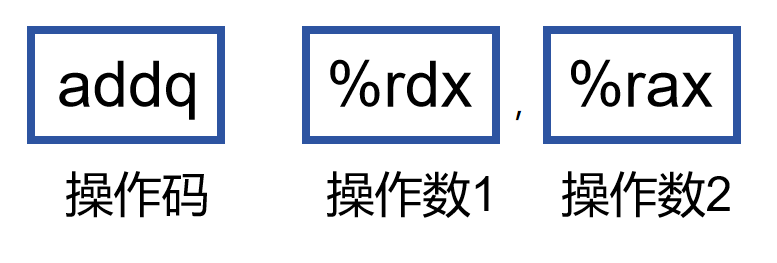
\includegraphics[width=0.8\textwidth]{figures/ass.png}
    \caption{汇编语句的组成}
    \label{fig:ass}
\end{figure}
编译器则是将源代码翻译为机器语言的工具,汇编语言作为机器语言的中间形式,提供了一种更易于理解和操作的方式。编译器的工作流程如\autoref{fig:compiler}所示。编译器会根据源代码构建一个语法树,然后根据语法树的规则转翻译源代码为汇编语言代码。不同版本的编译器在转译时有部分不同的处理方式,例如通过指令调度算法来减少跳转,寄存器换名技术来消除数据冲突。
\begin{figure}
    \centering
    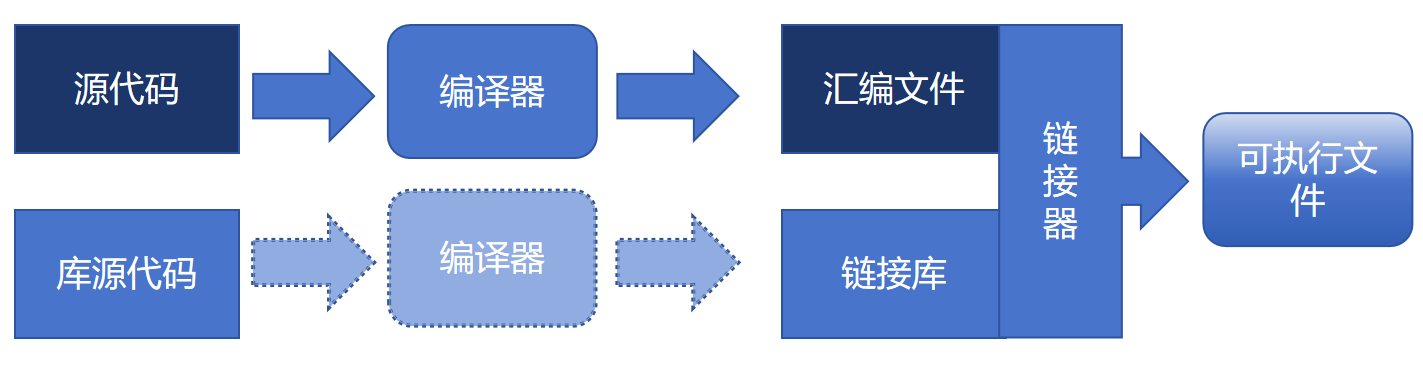
\includegraphics[width=0.8\textwidth]{figures/compiler.png}
    \caption{编译器的工作流程}
    \label{fig:compiler}
\end{figure}
随着编程语言的演变,编译器也在不断更新。例如,GCC(GNU Compiler Collection)已经更新到13.2.0版本。不同版本的编译器在编译同一程序时可能产生不同的编译结果;即使是相同版本的编译器,使用不同的编译选项也会导致编译结果的差异。因此,研究如何利用这些差异来区分编译器的版本具有重要意义。
\par
\subsection{问题重述}
\textbf{问题1}:使用多种不同版本的GCC C++编译器默认编译选项,编译附件中的程序源代码1。任务核心是对比这些不同版本编译器的输出结果,识别并记录体现编译器版本差异的特征。

\textbf{问题2}:将识别出的编译器版本特征转化为实际可用的判别函数。

\textbf{问题3}:使用不同版本的GCC C++编译器编译附件中的程序源代码2,应用已开发的判别函数测试其效果,验证其在不同源代码上的普适性和准确性,并研究更加广泛有效的判别函数。

\textbf{问题4}:提出几条建议以提高判别函数的性能,包括提升判别函数的区分度和增强对不同源代码的泛化能力。

\vspace*{1cm}
\section{问题分析}
\subsection{问题一分析}
问题一要求我们提取出不同版本GCC编译附件1结果中的主要特征,以用于构建判别函数。为此,我们首先利用Vs Code的文本比较工具,了解各个汇编文件的差异,之后编写程序实现对多个版本编译的汇编文件进行特征提取。我们将考虑提取操作码和寄存器的频率、Bigram(连续两个指令组合)的数量、代码块数量等特征,这些特征能更全面地反映不同版本编译器的行为差异。通过对这些特征的分析,我们为后续的问题二提供了坚实的数据基础。

\subsection{问题二分析}
在问题一的基础上,我们需要利用提取的特征数据构建判别函数。这是一个典型的多分类问题,特征数据将作为输入变量,不同的GCC版本作为标签类别。我们将使用机器学习算法,如Gini决策树、随机森林等,来构建判别模型。通过这些算法,我们能够实现不同版本GCC编译结果的有效分类和识别,并为后续的问题三提供强大的模型支持。

\subsection{问题三分析}
问题三要求利用构建的判别器对不同版本GCC编译附件2的结果进行版本预测。在这个阶段,我们将模型应用于未见过的数据上,以验证其普适性和准确性。考虑到数据集的规模和特征的复杂性,我们将使用交叉验证来评估模型的性能,并在必要时对模型进行改进,以提升其在附件2上的预测准确性。

\subsection{问题四分析}
为了进一步提升判别函数的性能,我们提出了以下改进建议:首先,可以尝试引入深度学习模型,进行自动特征提取,再基于如Transformer的注意力机制模型,以捕捉更复杂的特征关系;其次,增加数据集的多样性,涵盖不同类型、不同规模的源代码,并通过不同的编译优化级别生成更多样的训练数据;最后,通过结合静态和动态特征,使模型能够从多个维度进行学习和预测,从而提高模型的泛化能力和预测准确率。

\vspace*{1cm}
\section{模型假设}
\begin{enumerate}%创建有序列表
  \item 假设不同版本编译器对于实现同一功能,偏向于使用某些特定的操作码与寄存器。因为随着硬件的进步,指令更新,编译器将采用新的指令以实现更快的功能。
  \item 假设采用Windows下的mingw64进行编译源代码。因为附件1中的源代码含有easyx图形库,导致gcc无法在Linux系统下编译代码。所以我们考虑到既要能够编译,也要使用与gcc相关的编译器,故使用mingw64。
  \item 假设不提取汇编文件“.ident”的相关特征。无论是gcc还是mingw64采用默认编译出来的汇编文件,都含有“.ident”这一项,该项会直接注明汇编文件是由哪个版本的编译器生成的。我们考虑到实际应用中需要判别的是二进制文件,通过二进制文件反编译成汇编文件会失去'.ident'这个特征。
\end{enumerate}
\vspace*{1cm}
\renewcommand{\arraystretch}{1.5}
\section{符号说明}
\begin{table}[H]
\caption{\textbf{符号说明}}%标题
\centering%把表居中
\begin{tabular}{cc}%三列,内容全部居中
\toprule%第一道横线
 符号 &说明\\
\midrule%第二道横线
 D & 给定样本集合 \\
$p_i$ & 样本集中属于第i类的样本比例 \\
  C& 类的数量 \\
  $|D_{left}|$ & 划分后数据集$D_left$中样本的数量 \\
   $|D_{right}|$ & 划分后数据集$D_right$中样本的数量 \\
    $|D|$ & 数据集$D$中总样本的数量 \\
    $D_{not-missing}$&属性A有值的样本集\\
    $D_{missing}$&属性A有缺失值的样本集\\
     $Gini(D)$ & 数据集D的基尼指数 \\
     $Gini(D,A,t_i)$&数据集D经特征A的划分点划分后的基尼指数\\
     $T$&叶子节点个数\\
     $q(x)$&样本x在树中的叶子节点的索引\\
     $\omega$&叶子节点的权重\\
     $\gamma$&控制叶子节点个数的惩罚权重\\
     $\lambda$&控制叶子节点的惩罚权重\\
     $l$&单个样本的损失函数\\
     $\mathcal{L}$&总体损失函数\\
     $\Omega$&正则函数\\
\bottomrule%第三道横线
\end{tabular}
\end{table}
\vspace*{1cm}
\section{问题一}
\subsection{寻找特征}
根据附件提供的编译器版本信息,我们综合考量了各版本的使用情况和差异程度,选择了以下五个GCC版本作为识别对象:“8.4.0”、“10.2.0”、“11.3.0”、“12.2.0”和“13.2.0”。将程序源代码1分别由这五个版本的GCC编译器进行编译,生成对应的五个汇编文件。
我们利用VS Code自带的文本比较工具,对这五个汇编文件进行两两比对。VS Code的文本比较工具主要是基于‘Myers diff’算法实现,该算法是由Eugene Myers在1986年提出的一种广泛使用的最短编辑距离算法,专门用于计算两个序列(例如文本文件的行或字符)之间的最小修改步骤(插入、删除、替换)。
\begin{table}[H]
\caption{\textbf{8.4.0与10.2.0汇编指令对比}}%标题
\label{tab:zhiling}
\centering%把表居中
\begin{tabular}{l|l|l}%三列,内容全部居中

\toprule%第一道横线
\multicolumn{1}{c}{line} & \multicolumn{1}{c}{8.4.0} & \multicolumn{1}{c}{10.2.0} \\
\midrule%第二道横线 
1 &movl	252(\%rbp), \textcolor{red}{\%eax}&movl	252(\%rbp), \textcolor{blue}{\%edx} \\
  2 &\textcolor{red}{movslq	\%edx, \%rdx}&\textcolor{blue}{cltq}\\
3 &salq	\$4, \textcolor{red}{\%rdx}&salq	\$4, \textcolor{blue}{\%rax}\\
4 &leaq	272(\%rbp), \%rbx&leaq	272(\%rbp), \%rbx\\
5 &addq	\%rbx, \textcolor{red}{\%rdx}&addq	\%rbx, \textcolor{blue}{\%rax}\\
6 &subq	\$160, \textcolor{red}{\%rdx}&subq	\$160, \textcolor{blue}{\%rax}\\
7 &movl	\textcolor{red}{(\%rdx)}, \textcolor{red}{\%edx}&movl	\textcolor{blue}{(\%rax)}, \textcolor{blue}{\%eax}\\
8 &subl	\textcolor{red}{\%edx}, \textcolor{red}{\%eax}&subl	\textcolor{blue}{\%eax}, \textcolor{blue}{\%edx} \\
\bottomrule%第三道横线
\end{tabular}

\end{table}



\autoref{tab:zhiling}展示了由'8.4.0'和'10.2.0'版本的GCC编译器生成的汇编文件中的部分差异。从表中可以看出,主要差异集中在操作码和寄存器的使用上。因此,我们计划提取汇编文件中的操作码和寄存器的数量。此外,考虑到某些可能的关联特性,如操作码与寄存器、寄存器与寄存器之间的关系,我们还将提取Bigram的数量。其中Bigram(2-gram)是指连续两个词或字符的组合,例如 "I am a student" 的 bigram 为 ['I am', 'am a', 'a student']。
\begin{figure}
    \centering
    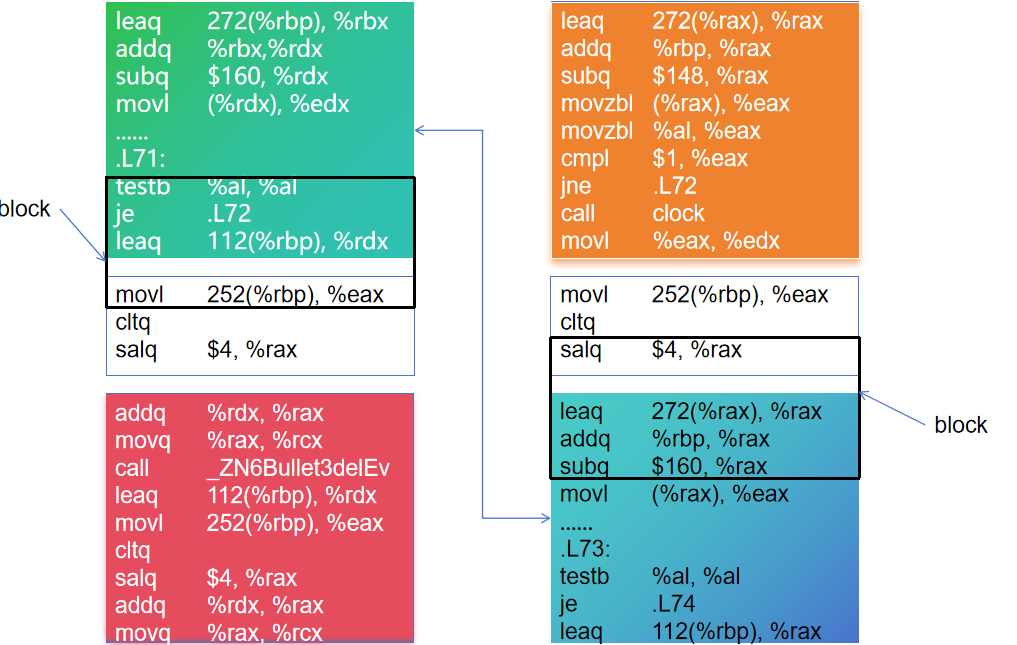
\includegraphics[width=1\linewidth]{figures/block.png}
    \caption{Enter Caption}
    \label{fig:block}
\end{figure}


  \autoref{fig:block}展示了由GCC编译器'10.2.0'和'12.2.0'版本生成的汇编文件中的部分差异。从图中可以清晰地看出,这些差异主要体现在汇编代码块的位置调度上。为了更好地捕捉这种位置特征,我们计划提取汇编代码中的block数量。这里的block指的是由连续的汇编指令组合而成的代码片段。经过多次实验验证,我们发现,当选择连续2条汇编指令作为block时,所提取的特征维度过高,导致分析复杂度增加;而当选择连续4条汇编指令时,提取到的特征维度过少,信息量不足。因此,经过综合考量,我们决定选择连续3条汇编指令的组合,认为这是在特征丰富度和维度可控性之间的最佳平衡点。

此外,在提取block数量时,为了捕捉更加广泛的特征,我们采用了一个细化的标准:当连续的汇编指令具有相同的操作码时,我们将这些指令视为属于同一个block。这样的方法能够更准确地反映代码块的内部结构,从而提升特征提取的精度。

  综上所述,我们最终决定将操作码、寄存器、Bigram以及block数量作为汇编文件的关键特征属性进行提取和分析。这些特征能够全面反映汇编文件中的结构和行为差异,为后续的模型训练和分析提供了丰富的信息基础。

  \subsection{提取特征}
  对汇编文件进行特征提取之前,为了获取更加泛化有效的特征,我们对其做了一些预处理。
  
  例如,在8.4.0版本GCC编译器生成的汇编文件中,指令'movl \$98, \%eax'与'movl \$1, \%eax'都表示将一个立即数移动到寄存器\%eax中,随后寄存器中的数值即为该立即数。为了消除这些指令中立即数的差异性,我们将汇编文件中的所有立即数统一替换为\$0,使得替换后的汇编指令形如'movl \$0, \%eax'。对于指令'movl -12(\%rbp), \%eax'与'movl -20(\%rbp), \%eax',两者都表示将位于基址寄存器\%rbp偏移一定字节的内存地址中的32位数据读取到寄存器\%eax中。因此,我们统一将这些指令中的偏移量删除,替换后的汇编指令形如'movl (\%rbp), \%eax'。这种预处理方法能够减少汇编指令的多样性,聚焦于更具普遍性的特征,从而提高特征提取的效果。

  通过上述方法对汇编文件进行预处理,我们在保持其基本语义完整的前提下,能够更加有效地提取出更多相关的特征。具体来说,这些预处理步骤不仅规范了汇编指令的表示形式,还减少了特征的多样性,使得后续的特征提取和分析更加精准和高效。这种预处理方式有助于在特征选择和模型训练过程中,突出重要的特征关联,同时避免因不必要的语法差异而带来的干扰,从而提升模型的整体表现和分析的准确性。

  我们将对生成的五个汇编文件进行特征提取,最终获得的数据规模为5*428,这意味着每个汇编文件包含428个特征。由于特征维度较大,为了便于分析和展示,我们将选择前50个特征数据,并使用热力图进行可视化。通过这种方式,我们可以更直观地观察和比较各汇编文件在这些特征维度上的差异和相似性,从而为后续的数据分析提供有价值的参考。
  \begin{figure}
      \centering
      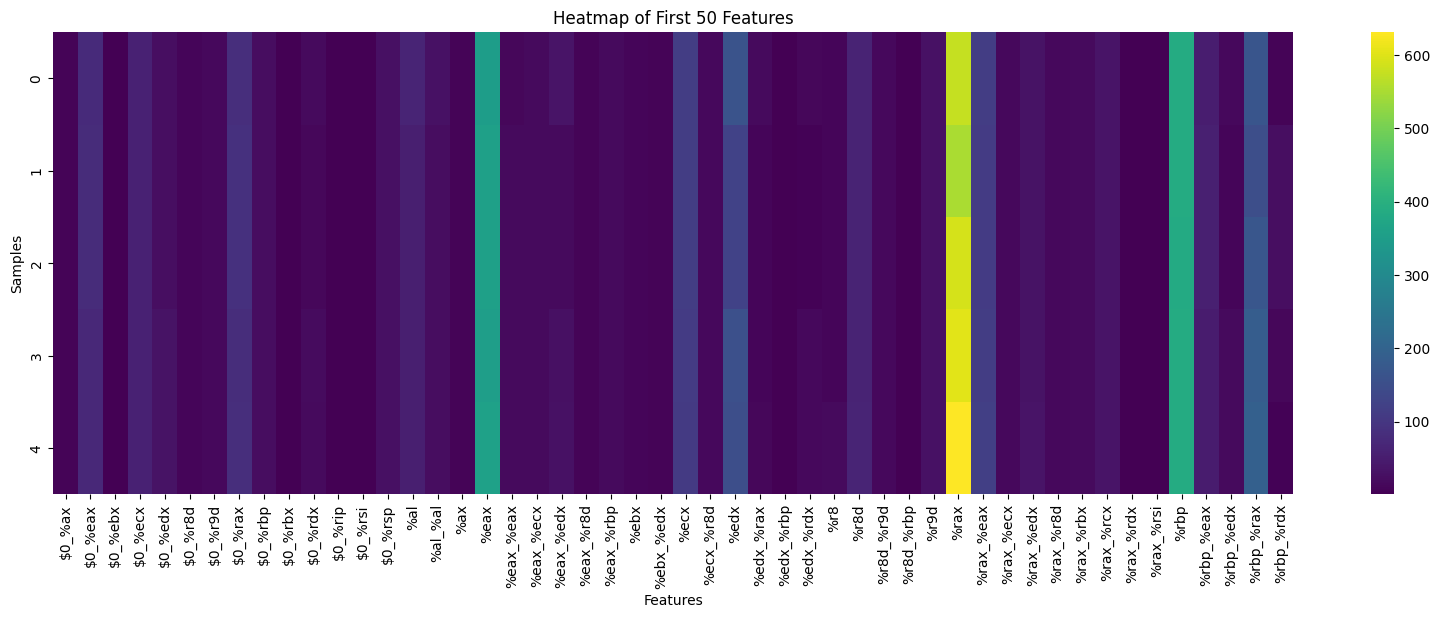
\includegraphics[width=1\linewidth]{figures/same.png}
      \caption{Enter Caption}
      \label{fig:same}
  \end{figure}


从\autoref{fig:same}可以看出,五个汇编文件在某些特征维度上的取值大致相同。鉴于此,我们决定对数据进行降维处理,将这些取值相同的特征去除。这样做有两个主要原因:一方面,减少特征维度可以降低模型的计算复杂度,简化模型的训练过程;另一方面,取值相同的特征对我们后续的版本判别并无实际帮助。因此,在降维之后,我们最终获得了规模为5*89的数据集,这意味着共有339个特征的取值是相同的,并已被剔除。最终获取的数据结果如\autoref{tab:feature}所示:
\begin{table}[H]
\caption{\textbf{特征数据}}%标题
\label{tab:feature}
\centering%把表居中
\begin{tabular}{lccccc}%三列,内容全部居中
\toprule%第一道横线
 feature\_name&8.4.0 & 10.2.0 & 11.3.0 & 12.2.0 & 13.2.0 \\ 
\midrule%第二道横线 
\$0\_\%eax&77&78&78&72&72 \\
\$0\_\%edx&25 & 25 & 25 & 31 & 31 \\
\$0\_\%rax&84 & 89 & 89 & 80 & 84 \\
\$0\_\%rdx&17 & 12 & 12 & 19 & 17 \\
\%al2 & 64 & 55 & 55 & 55&55 \\
...&... & ... & ... & ... & ... \\
testb&30 & 21 & 21 & 21 & 21 \\
testb\_\%al&30 & 21 & 21 & 21 & 21 \\
testb\_je\_leaq&9 & 8 & 8 & 8 & 8 \\
testl&2 & 6 & 6 & 6 & 6 \\
testl\_\%eax&2 & 6 & 6 & 6 & 6 \\
\bottomrule%第三道横线
\end{tabular}
\end{table}
   

\vspace*{1cm}
\section{问题二模型的建立与求解}
  \subsection{数据分析}
  我们对部分特征数据的分布进行了可视化,结果如\autoref{fig
}所示。图中展示了不同版本GCC编译器生成的汇编文件在操作码、寄存器、Bigram与block数量上的分布情况。可以明显看出,不同版本的编译器在这些特征上存在一定的差异,这些差异正是我们判断编译器版本的重要依据。通过分析这些特征的分布,我们能够更准确地捕捉到各个编译器版本之间的区别,为后续的模型训练和分析提供了有力的支持。
  \begin{figure}[H]
      \centering
      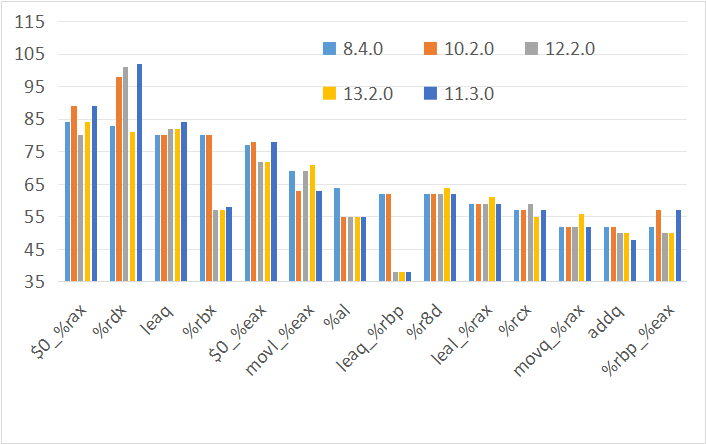
\includegraphics[width=1\linewidth]{figures/hist.png}
      \caption{Enter Caption}
      \label{fig:hist}
  \end{figure}

  
计算各个特征与标签的皮尔逊相关系数(Pearson Correlation Coefficient),该系数适用于衡量两个连续变量之间的线性关系。皮尔逊相关系数的计算公式为
\begin{equation}
\rho_{X,Y} = \frac{\text{cov}(X, Y)}{\sigma_X \sigma_Y}
\label{eq:correlation}
\end{equation}

其中,协方差 \(\text{cov}(X, Y)\) 的计算公式为:
\begin{equation}
\text{cov}(X, Y) = \frac{1}{n} \sum_{i=1}^{n} (X_i - \mu_X)(Y_i - \mu_Y)
\label{eq:covariance}
\end{equation}

标准差 \(\sigma_X\) 和 \(\sigma_Y\) 的计算公式为:
\begin{equation}
\sigma_X = \sqrt{\frac{1}{n} \sum_{i=1}^{n} (X_i - \mu_X)^2}
\label{eq:stddev_x}
\end{equation}
\begin{equation}
\sigma_Y = \sqrt{\frac{1}{n} \sum_{i=1}^{n} (Y_i - \mu_Y)^2}
\label{eq:stddev_y}
\end{equation}

均值 \(\mu_X\) 和 \(\mu_Y\) 的计算公式为:
\begin{equation}
\mu_X = \frac{1}{n} \sum_{i=1}^{n} X_i
\label{eq:mean_x}
\end{equation}
\begin{equation}
\mu_Y = \frac{1}{n} \sum_{i=1}^{n} Y_i
\label{eq:mean_y}
\end{equation}

  \begin{figure}[H]
      \centering
      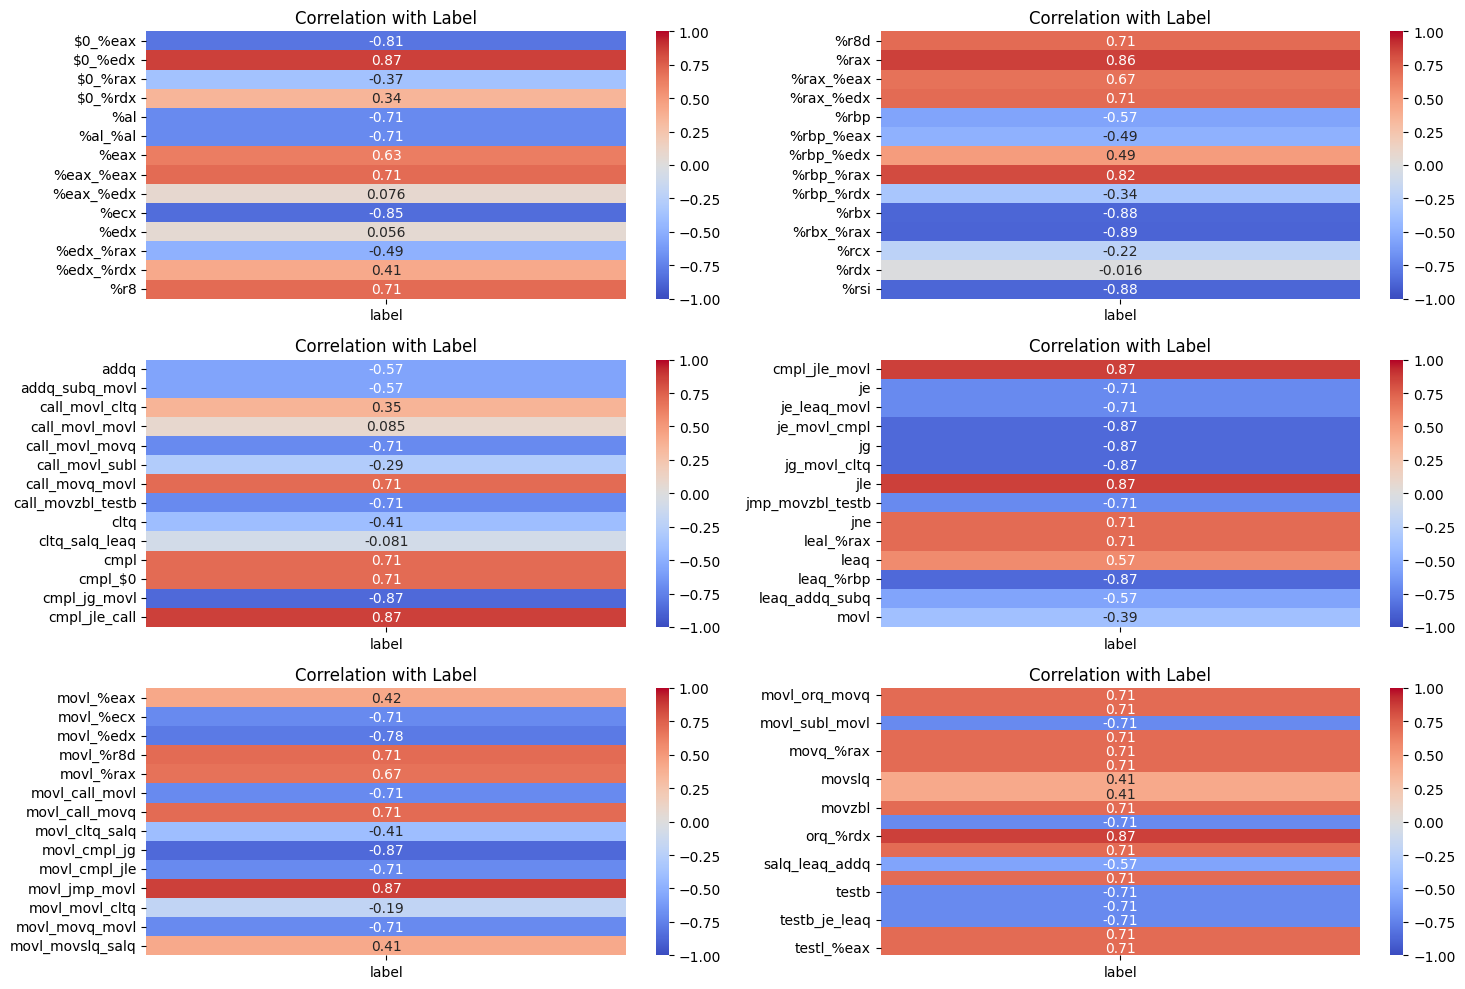
\includegraphics[width=1\linewidth]{figures/corr.png}
      \caption{特征与标签的皮尔逊相关系数}
      \label{fig:corr}
  \end{figure}
我们得到了如\autoref{fig
}所示的结果。虽然图中显示部分特征之间的相关系数较高,但我们对这些相关性进行了统计显著性检验。具体来说,我们设立了原假设$H_0$,即“两个变量之间不存在显著的线性关系”;同时,备择假设$H_1$为“两个变量之间存在显著的线性关系”。通过对相关系数进行显著性检验,我们能够更准确地判断变量之间的关系,从而为模型的构建提供更可靠的依据。

我们使用t 统计量来进行相关系数检验。t 统计量的计算公式为:
\begin{equation}
t = \frac{r \sqrt{n - 2}}{\sqrt{1 - r^2}}
\label{eq:t}
\end{equation}
其中:
\begin{itemize}
    \item \(r\) 是计算得到的 Pearson 相关系数。
    \item \(n\) 是样本量。
    \item t 统计量服从自由度为 \(n - 2\) 的 t 分布。
\end{itemize}
计算得到 t 统计量后,可以通过查找 t 分布表或使用计算工具来找到对应的 p 值。p 值是与 t 统计量对应的累积概率值,表示在原假设为真的情况下,t 统计量出现当前值或更极端值的概率。对于p值的解释是:
\begin{itemize}
    \item \textbf{低 p 值(通常 < 0.05)}:意味着在原假设为真的情况下,观察到当前相关系数的概率非常低,因此我们有理由拒绝原假设,认为相关系数是显著的。
    \item \textbf{高 p 值(通常 ≥ 0.05)}:意味着在原假设为真的情况下,观察到当前相关系数的概率较高,因此我们无法拒绝原假设,认为相关系数可能不是显著的。
\end{itemize}
从\autoref{fig:p}中可以看到,几乎所有特征属性的$p$值都大于显著性水平$\alpha = 0.05$,因此我们不拒绝原假设,即认为这些特征之间的相关系数可能是由于随机误差引起的。这一结果可能是因为每类数据样本中仅包含一个观测值,因此这些特征不具备统计显著性。这表明在这些特征中,无法确认显著的线性关系,因此它们对线性模型的贡献可能较为有限。这也提示我们需要进一步分析,或考虑选择其他适合的模型来更好地捕捉数据中的关系。
\begin{figure}[H]
    \centering
    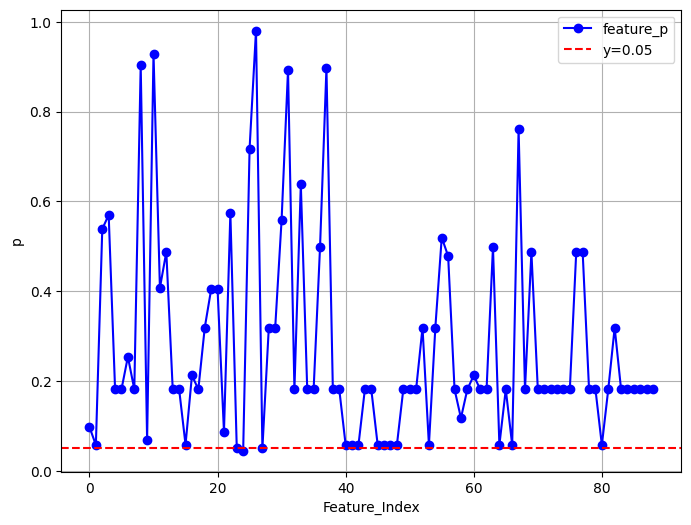
\includegraphics[width=0.75\linewidth]{figures/p.png}
    \caption{统计显著性水平}
    \label{fig:p}
\end{figure}
 
  
  因此我们接着计算了特征属性与标签的互信息。由于我们的标签是离散属性,而特征是连续属性。所以我们将特征进行离散化处理,以便于计算互信息。互信息衡量了两个随机变量之间的“信息共享”量。如果两个随机变量 $X$ 和 $Y$ 是独立的,那么它们之间的互信息为零,表示知道一个变量不会提供关于另一个变量的任何信息。如果互信息较大,则表示两个变量之间有较强的依赖关系。
 
对于两个离散随机变量 \(X\) 和 \(Y\),互信息定义为:
\begin{equation}
I(X; Y) = \sum_{y \in Y} \sum_{x \in X} p(x, y) \log \left(\frac{p(x, y)}{p(x) p(y)}\right)
\label{eq:mutual_information}
\end{equation}

互信息还可以通过熵来表示:
\begin{equation}
I(X; Y) = H(X) + H(Y) - H(X, Y)
\label{eq:mutual_information_entropy}
\end{equation}

其中,各个熵的计算公式为:
\begin{equation}
H(X) = -\sum_{x \in X} p(x) \log p(x)
\label{eq:entropy_x}
\end{equation}

\begin{equation}
H(Y) = -\sum_{y \in Y} p(y) \log p(y)
\label{eq:entropy_y}
\end{equation}

\begin{equation}
H(X, Y) = -\sum_{x \in X} \sum_{y \in Y} p(x, y) \log p(x, y)
\label{eq:joint_entropy}
\end{equation}
\begin{figure}[H]
      \centering
      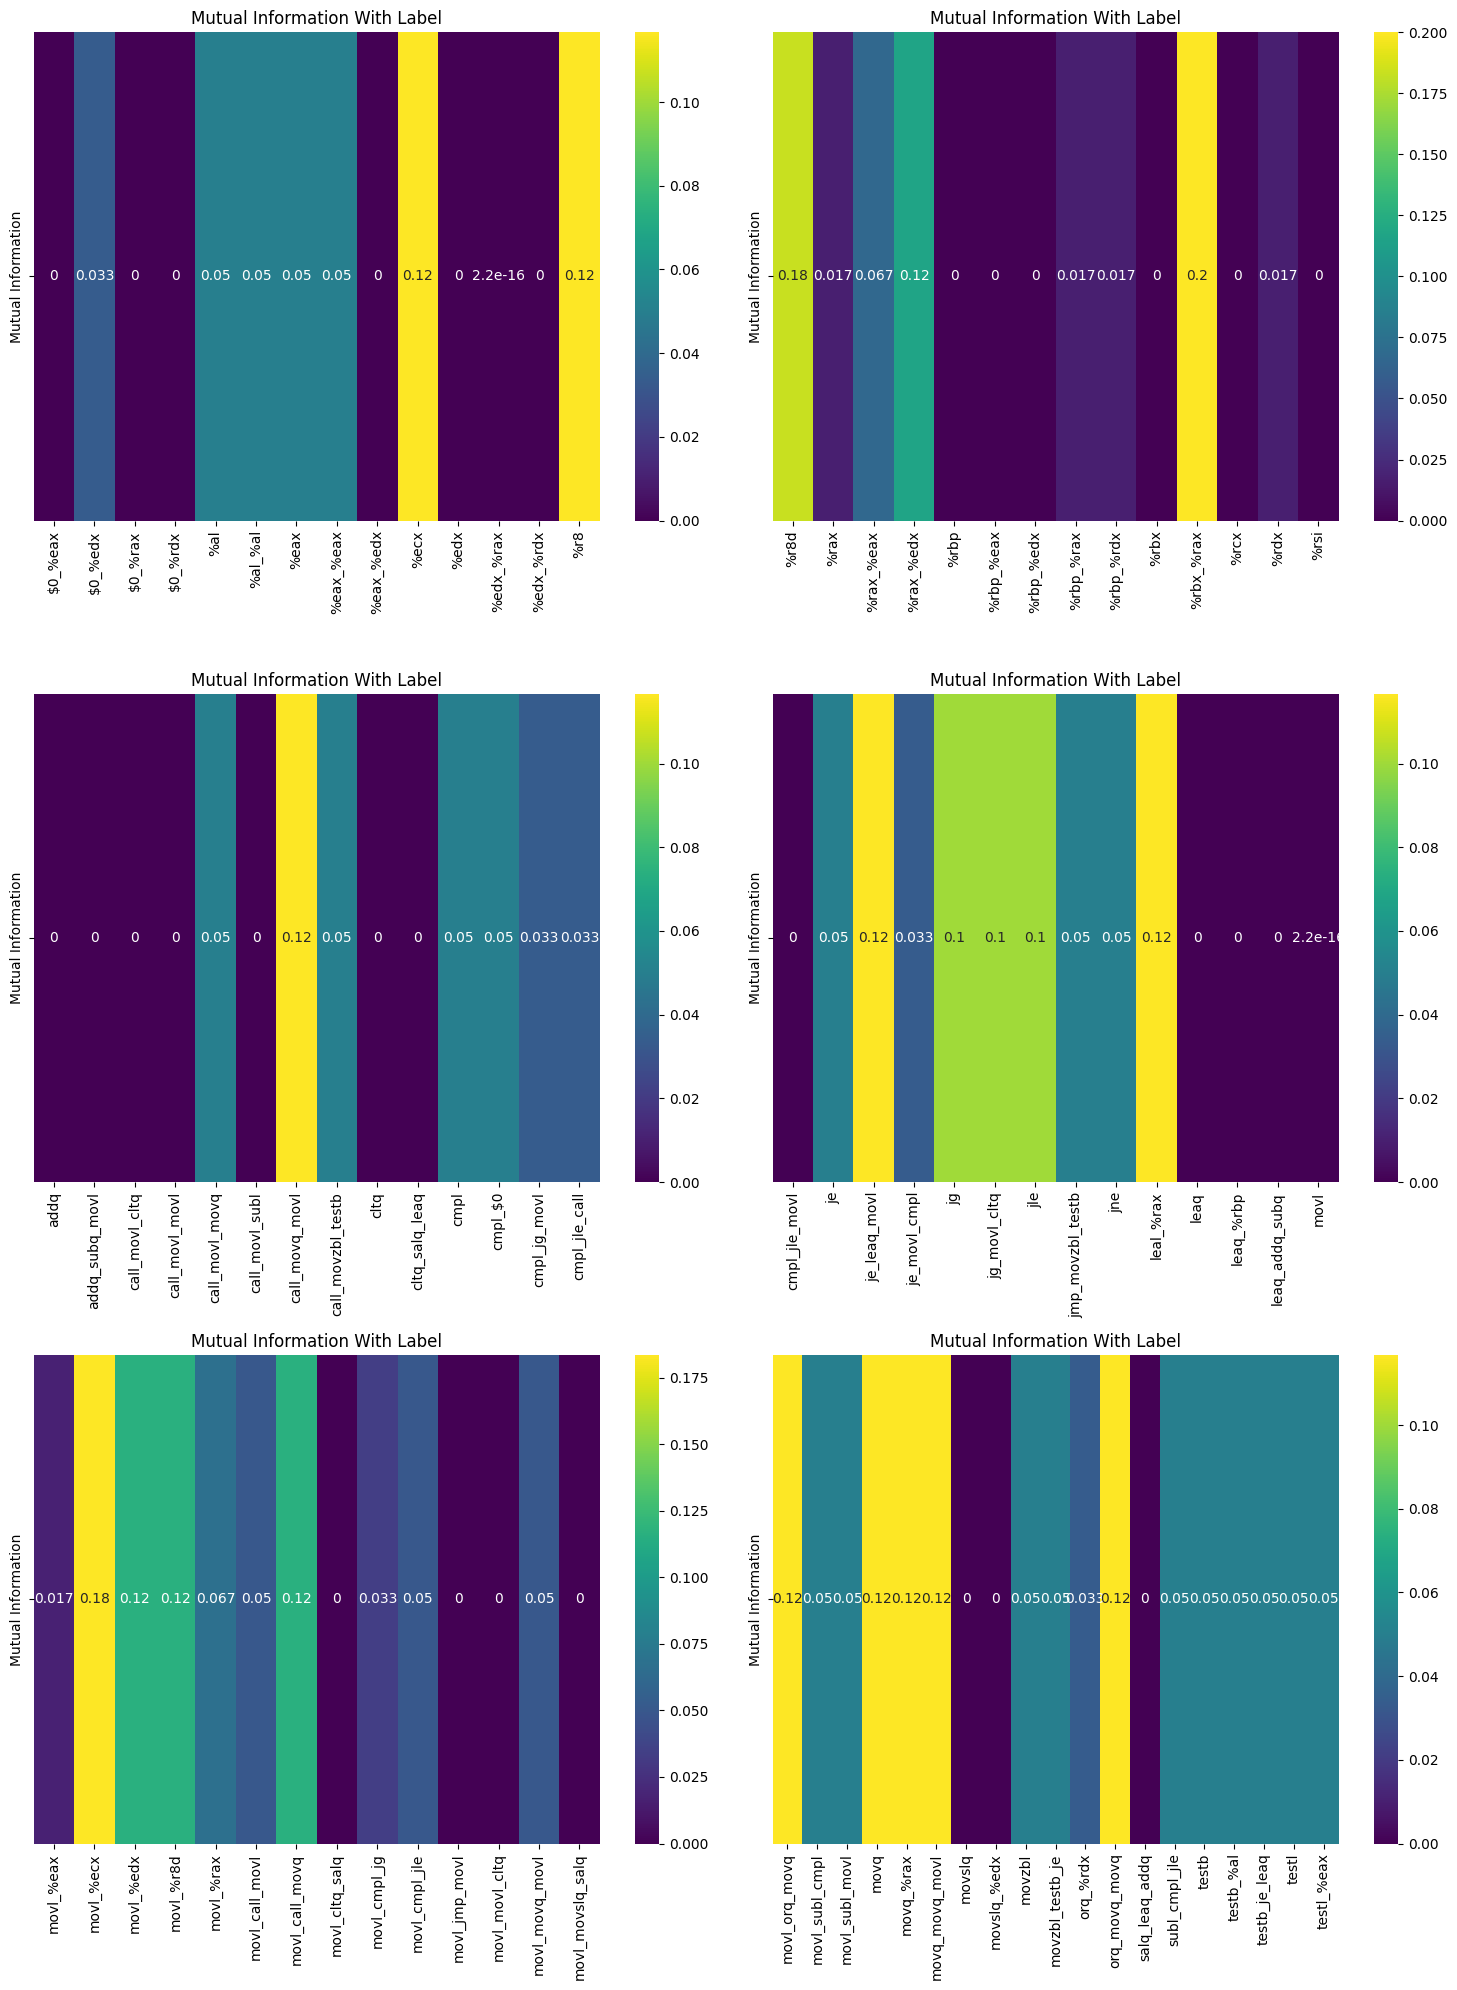
\includegraphics[width=0.75\linewidth]{figures/Information.png}
      \caption{特征与标签的互信息}
      \label{fig:Information}
  \end{figure}
从\autoref{fig:Information}中我们可以得到如下信息:
\begin{itemize}
    \item 高互信息的特征:互信息值高的特征(如 '\%edx\_\%eax'、'\%r8d'、'cmp\_jle\_movl' 等)在图中以黄色或绿色显示,这些特征是我们在模型中特别需要关注的,因为它们对标签具有较高的预测能力。
    \item 低互信息或零互信息的特征:互信息值为零或接近零的特征对标签几乎没有贡献,可以考虑在特征选择过程中进行剔除或降低其权重,以简化模型。
    \item 互信息的分布:从图中可以看出,互信息较高的特征集中在一些特定的寄存器组合或指令组合上,这表明这些组合对于模型预测特别重要。基于此,我们可以重点关注这些特征,并在模型训练中对其进行优化。
\end{itemize}

因此,基于数据分析和文献阅读的结果,我们推测特征属性与编译器版本之间的关系可能是非线性的。鉴于我们的数据为连续值,并且考虑到不同源代码生成的汇编文件可能表现出不同的特征属性,我们的模型需要具备处理含有缺失值的数据的能力。经过综合考量,我们决定采用Gini决策树模型,因为它能够很好地支持上述特性,适应非线性关系,并且在面对缺失数据时依然能进行有效的预测。
    \subsection{模型说明}
    \subsubsection{Gini系数的计算}
gini系数的定义是样本属于不同类的概率之和,用于衡量纯度。对于给定的样本集合 \(D\),Gini系数可以表示为:
\begin{equation}
Gini(D) = 1 - \sum_{i=1}^{C} p_i^2
\end{equation}
其中:
\begin{itemize}
  \item \(p_i\) 是样本集中第 \(i\) 类的样本比例(即属于第 \(i\) 类的样本数量占总样本数量的比例)。
  \item \(C\) 是类别的数量。
\end{itemize}





\subsubsection{连续属性划分点t的确定}

\paragraph{排序连续属性的值}
对于一个连续属性 \(A\),首先对所有样本的该属性值进行排序。假设排序后的值为 \(a_1, a_2, \dots, a_n\),其中 \(a_i\) 是第 \(i\) 个样本在属性 \(A\) 上的取值,并且满足 \(a_1 \leq a_2 \leq \dots \leq a_n\)。

\paragraph{候选划分点的确定}
候选划分点 \(t_i\) 通常选在两个相邻样本值的中间,即:
\begin{equation}
t_i = \frac{a_i + a_{i+1}}{2}, \quad i = 1, 2, \dots, n-1
\end{equation}

\paragraph{计算每个划分点的Gini指数}
对于每个候选划分点 \(t_i\),将数据集 \(D\) 分为两个子集 \(D_{\text{left}}\) 和 \(D_{\text{right}}\):
\begin{equation}
D_{\text{left}} = \{x \in D \mid A(x) \leq t_i\}
\end{equation}
\begin{equation}
D_{\text{right}} = \{x \in D \mid A(x) > t_i\}
\end{equation}

然后计算基于划分点 \(t_i\) 的Gini指数:
\begin{equation}
Gini(D, A, t_i) = \frac{|D_{\text{left}}|}{|D|} Gini(D_{\text{left}}) + \frac{|D_{\text{right}}|}{|D|} Gini(D_{\text{right}})
\end{equation}
其中:
\begin{itemize}
  \item \(|D_{\text{left}}|\) 和 \(|D_{\text{right}}|\) 是两个子集的样本数量。
  \item \(Gini(D_{\text{left}})\) 和 \(Gini(D_{\text{right}})\) 分别是两个子集的Gini系数。
  \item \(|D|\) 是样本集 \(D\) 的总样本数量。
\end{itemize}
\paragraph{选择最优划分点}
最优划分点 \(t^*\) 是使得Gini指数最小的划分点:
\begin{equation}
t^* = \arg\min_{t_i} Gini(D, A, t_i)
\end{equation}

通过此方法,我们得到了最优的划分点 \(t^*\),并将其用于决策树的构建。






\subsubsection{处理连续属性}
对于连续属性 \(A\),通过划分点 \(t\) 将样本集 \(D\) 划分为两个子集:\(D_{\text{left}}\) 和 \(D_{\text{right}}\),分别表示小于等于 \(t\) 和大于 \(t\) 的样本集。划分后的Gini指数为:
\begin{equation}
Gini(D, A, t) = \frac{|D_{\text{left}}|}{|D|} Gini(D_{\text{left}}) + \frac{|D_{\text{right}}|}{|D|} Gini(D_{\text{right}})
\end{equation}


\subsubsection{处理缺失值}
对于属性 \(A\) 存在缺失值的情况,假设缺失值比例为 \(p_{\text{missing}}\),则Gini系数可以表示为:
\begin{equation}
Gini(D, A) = (1 - p_{\text{missing}}) \times Gini(D_{\text{not-missing}}, A) + p_{\text{missing}} \times Gini(D_{\text{missing}})
\end{equation}
其中:
\begin{itemize}
  \item \(D_{\text{not-missing}}\) 是属性 \(A\) 有值的样本集。
  \item \(D_{\text{missing}}\) 是属性 \(A\) 缺失值的样本集。
  \item \(Gini(D_{\text{not-missing}}, A)\) 和 \(Gini(D_{\text{missing}})\) 分别是有值样本集和缺失值样本集的Gini系数。
\end{itemize}

\subsubsection{选择最优划分}
在考虑了所有可能的划分点 \(t\) 以及缺失值的影响后,选择使得Gini指数最小的划分点作为最终的划分点,以确保在当前节点上的样本被分成更加纯净的子集。

\subsubsection{构建树结构}
在找到最优划分后,决策树会在此处创建一个分裂节点,并将数据集分成左右子集。然后递归地对每个子集重复上述步骤,直到满足停止条件为止。

\subsection{模型建立}
Gini决策树的伪代码如下:
\begin{algorithm}[H]
    \caption{决策树构建算法}
    \label{alg:decision_tree}
    \begin{algorithmic}
        \REQUIRE 数据集 $D$,属性集 $A$,停止条件
        \ENSURE 决策树

        \STATE \textbf{函数} \texttt{BuildTree}($D$, $A$):
        \STATE \quad \textbf{If} 所有样本都属于同一类 \textbf{Then}
        \STATE \quad \quad 将当前节点标记为该类,返回
        \STATE \quad \textbf{If} 属性集为空或满足停止条件 \textbf{Then}
        \STATE \quad \quad 将当前节点标记为样本中最多的类,返回
        \STATE \quad \textbf{For each} 属性 $A_i \in A$ \textbf{Do}
        \STATE \quad \quad \textbf{If} $A_i$ 是连续属性 \textbf{Then}
        \STATE \quad \quad \quad 对 $A_i$ 的值进行排序
        \STATE \quad \quad \quad 计算每个候选划分点 $t_i = \frac{a_i + a_{i+1}}{2}$
        \STATE \quad \quad \quad 对每个候选划分点 $t_i$ 计算 Gini 指数
        \STATE \quad \quad \textbf{Else If} $A_i$ 有缺失值 \textbf{Then}
        \STATE \quad \quad \quad 计算 Gini 指数,考虑缺失值比例 $p_{\text{missing}}$
        \STATE \quad \quad \textbf{Else}
        \STATE \quad \quad \quad 计算每个可能划分的 Gini 指数
        \STATE \quad 选择使 Gini 指数最小的属性 $A^*$ 及其最优划分点 $t^*$
        \STATE \quad 将当前节点标记为 $A^*$ 的分裂节点
        \STATE \quad 根据划分点 $t^*$ 将样本集 $D$ 分为 $D_{\text{left}}$ 和 $D_{\text{right}}$
        \STATE \quad 递归调用 \texttt{BuildTree}($D_{\text{left}}$, $A$) 和 \texttt{BuildTree}($D_{\text{right}}$, $A$)
        
        \STATE \textbf{End Function}
    \end{algorithmic}
\end{algorithm}
基于伪代码\autoref{alg:decision_tree},我们构建了一颗Gini决策树,如\autoref{fig:Ginitree}所示:
\begin{figure}[H]
    \centering
    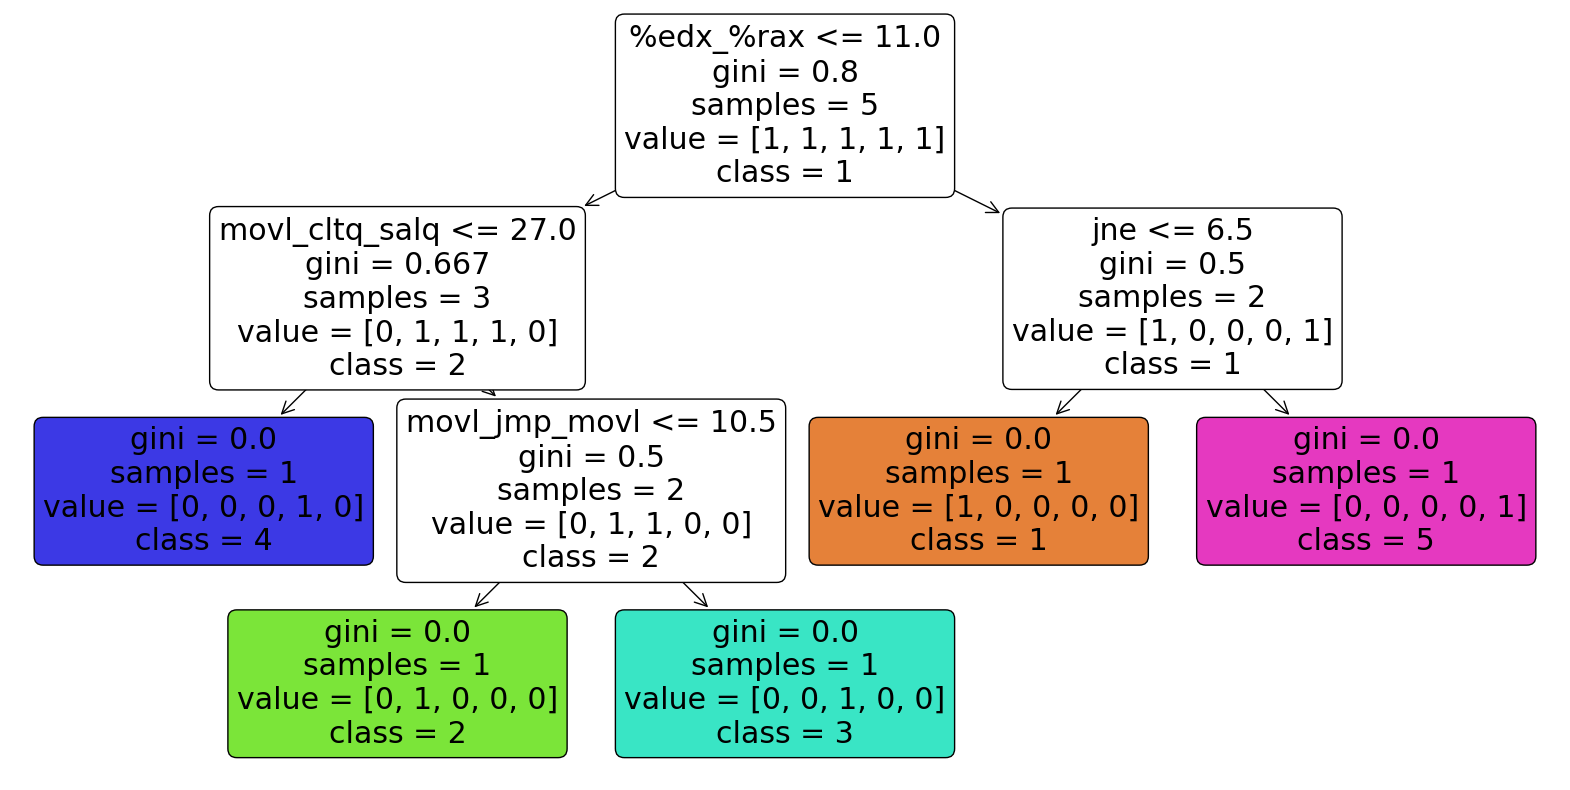
\includegraphics[width=1\linewidth]{figures/Ginitree.png}
    \caption{Gini决策树}
    \label{fig:Ginitree}
\end{figure}
这就是我们基于程序源代码1提取到的特征构建的判别函数。

\vspace*{1cm}

\section{问题3}
\subsection{决策树模型分析}
决策树模型作为一种简单且直观的机器学习算法,广泛应用于分类和回归任务。然而,尽管其易于理解和解释,决策树模型也存在一些固有的缺陷,决策树模型存在以下几个缺陷:
\begin{itemize}
	\item 容易过拟合:决策树模型在处理复杂数据集时,容易出现过拟合问题。这是因为决策树模型在构建过程中会根据数据的分布来选择分裂点,如果数据集过于复杂,决策树可能会生成\textbf{过深的树结构},从而导致模型过拟合,泛化能力较差。

	      \tbox{\autoref{fig:fit_status}展示了不同拟合状态的大致情况,过拟合是模型完全拟合了训练数据,把训练的数据的噪声也当做数据的统计特征,从而导致在训练集的误差很低,但是在测试集的误差很高。}
	\item 对数据噪声敏感:决策树对数据中的噪声和异常值非常敏感。这是因为决策树在构建过程中会根据数据的分布来选择分裂点,噪声和异常值可能导致树的结构发生较大变化,从而影响模型的稳定性和准确性。
	\item 不稳定:由于决策树的构建过程是基于局部最优的贪心算法,因此对数据的变化非常敏感,小的输入数据变化可能导致决策树结构的显著变化。
	\item 计算复杂度:在特征数量较多或数据集较大时,决策树的构建过程可能会非常耗时。这是因为每次分裂都需要计算所有可能分裂点的增益,从而选择最佳分裂点。
\end{itemize}
\begin{figure}[H]
	\centering
	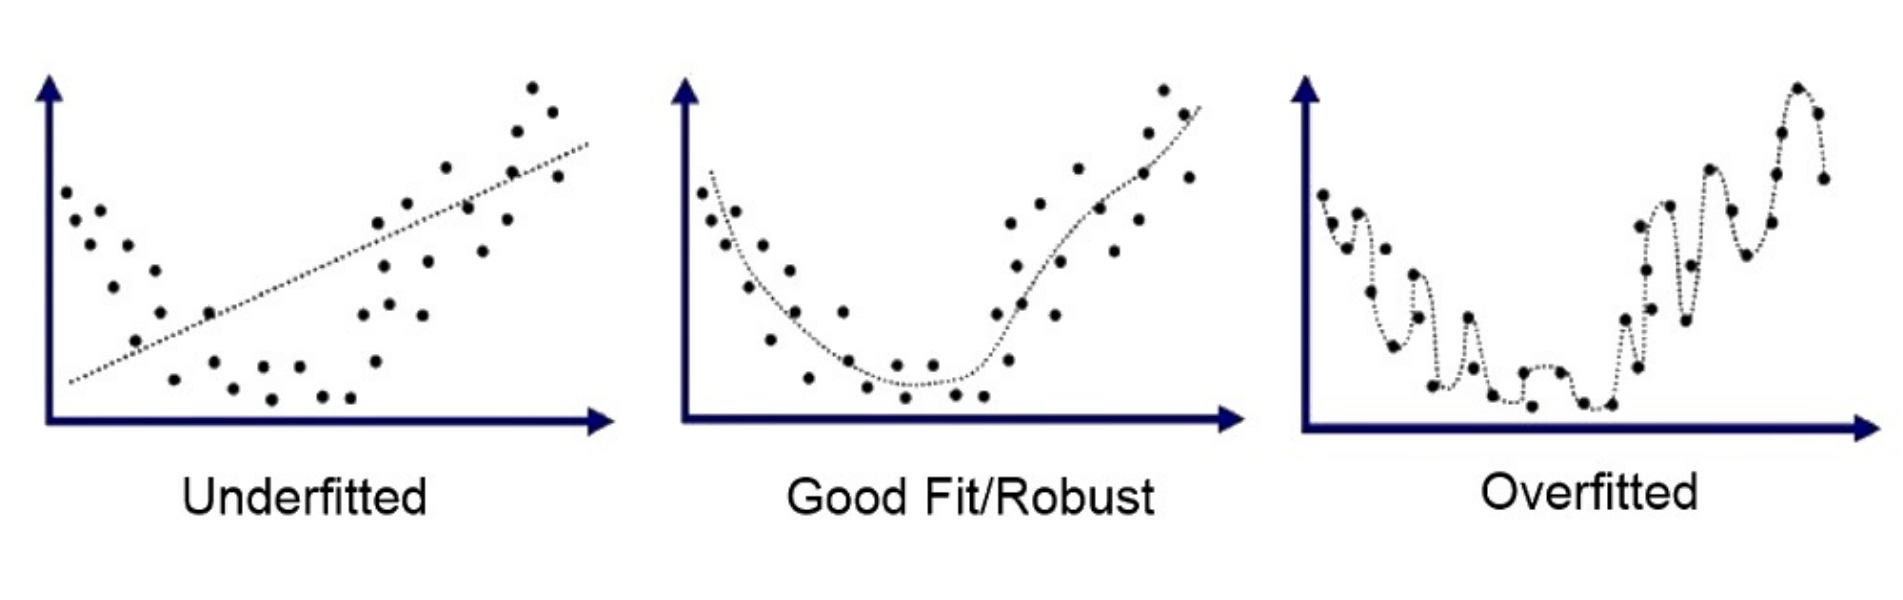
\includegraphics[width=0.8\textwidth]{figures/fit_status.png}
	\caption{不同拟合状态}
	\label{fig:fit_status}
\end{figure}

并且,在我们的实验中,我们发现如果只使用附件1或者是附件2来构建模型,模型的预测结果将会趋向于随机猜测,而非根据编译器的特征进行预测。
\par
从数据的分布来看,我们使用t-SNE算法对数据进行降维可视化,t-分布邻域嵌入(t-distributed Stochastic Neighbor Embedding,t-SNE)\cite{JMLR:v9:vandermaaten08a}是一种非线性降维技术,特别适用于高维数据的可视化。t-SNE通过将高维数据映射到低维空间,同时\textbf{尽可能保持数据点之间的局部结构},从而揭示数据的内在结构和模式。t-ESN算法通过优化KL散读来最小化高维空间和低维空间之间的分布差异,从而实现降维。t-SNE的优化目标是最小化高维空间和低维空间之间的KL散度,KL散度定义如下:
\begin{equation}
	C=KL(P||Q)=\sum_i\sum_jp_{ij}\log\frac{p_{ij}}{q_{ij}},
\end{equation}
其中,$p_{ij}$是高维数据点$x_i$和$x_j$之间的相似度,在高纬空间中,t-SNE算法使用高斯分布来衡量高维空间中点对之间的相似性。$q_{ij}$是低维数据点$y_i$和$y_j$之间的相似度。在低维空间中,t-SNE使用学生t分布(t-distribution)来计算点对之间的相似性。这个分布的长尾特性使得它能够更好地捕捉低维空间中的局部结构。t-SNE通过梯度下降算法优化该目标,C对于低维数据的梯度为
\begin{equation}
	\frac{\delta C}{\delta y_i}=4\sum_j(p_{ij}-q_{ij})(y_i-y_j)\left(1+\|y_i-y_j\|^2\right)^{-1},
\end{equation}
最后使用梯度更新低维数据点$y_i$
\begin{equation}
	y_i^{(t+1)}=y_i^{(t)}+\eta\frac{\delta C}{\delta y_i},
\end{equation}
其中$\eta$是学习率。在t-SNE算法中,还引入了\textbf{动量}来进一步优化低位数据点的表示:
\begin{equation}
	momentum=\alpha(y_i^{(t)}-y_i^{(t-1)}).
\end{equation}
动量项通过在更新过程中加入前几次更新的累积效果,可以帮助算法在梯度方向上更快地移动,并且通过平滑更新路径,能够有效减少震荡,使得优化过程更加稳定。加入动量后的更新公式为
\begin{equation}
	y_i^{(t+1)}=y_i^{(t)}+\eta\frac{\delta C}{\delta y_i}+\alpha(y_i^{(t)}-y_i^{(t-1)})m
\end{equation}
综上所述,T-SNE算法流程如\autoref{alg:tsne}所示。
\begin{algorithm}[H]
	\caption{t-SNE}
	\label{alg:tsne}
	\begin{algorithmic}
		\REQUIRE 数据集$X$,目标维度$k$,,优化参数:迭代次数$T$,学习率$\eta$,动量参数$\alpha$
		\ENSURE  低维数据$\mathcal{Y}$

		\STATE 计算高维数据之间的相似度$p_{j|
					i}$
		\[
		p_{j|i}=\frac{\exp\left(-\|x_i-x_j\|^2/2\sigma_i^2\right)}{\sum_{k\neq i}\exp\left(-\|x_i-x_k\|^2/2\sigma_i^2\right)}
		\]
		其中$\sigma_i$是以$\boldsymbol{x_i}$为中心的高斯分布的方差,通过二分搜索确定
		\STATE 从$\mathcal{N}(0,10^{-4}I)$从采样$\mathcal{Y}^{(0)}={y_1,y_2,\cdots,y_n}$
		\FOR {$i=1$ to $T$}
		\STATE 计算低维数据之间的相似度$q_{j|i}$
		\[q_{j|i}=\frac{(1+\|y_i-y_j\|^2)^{-1}}{\sum_{k\neq i}(1+\|y_i-y_k\|^2)^{-1}}\]
		\STATE 计算梯度
		\[
			\frac{\delta C}{\delta y_i}=4\sum_j(p_{ij}-q_{ij})(y_i-y_j)\left(1+\|y_i-y_j\|^2\right)^{-1}.
		\]
		\STATE 更新$y_i$
		\[
			y_i^{(t+1)}=y_i^{(t)}+\eta\frac{\delta C}{\delta y_i}+\alpha(y_i^{(t)}-y_i^{(t-1)})
		\]
		\ENDFOR
	\end{algorithmic}
\end{algorithm}
我们使用Scikit-learn\cite{scikit-learn}实现t-SNE算法的可视化,结果如\autoref{fig:tsne}所示。
\begin{figure}[H]
	\centering
	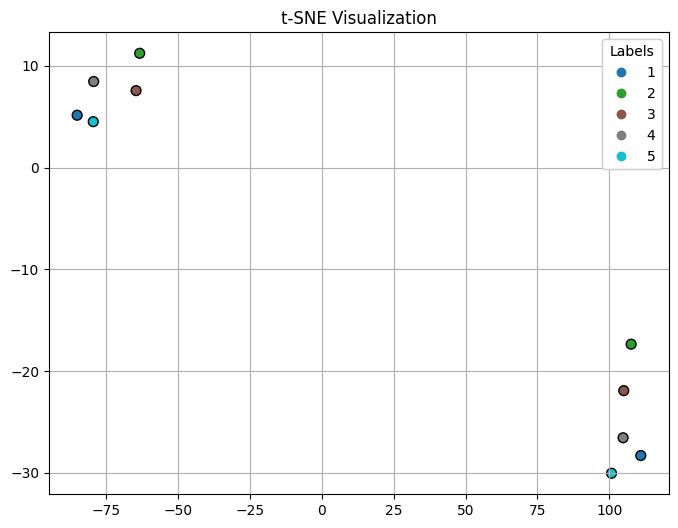
\includegraphics[width=0.7\textwidth]{figures/tsne.png}
	\caption{t-SNE降维可视化}
	\label{fig:tsne}
\end{figure}
可以发现,附件1和附件2在整体上的数据分布相差很远,并且在局部上同一个源文件的不同版本之间也没有明显的分布规律。这也是导致决策树模型无法准确预测的原因之一。
\vspace{1cm}
\subsection{模型改进}
通过对决策树模型和数据分布的分析,我们发现以下问题
\begin{itemize}
	\item \textbf{训练数据不具备广泛性}:原有的训练数据少,并且类型单一,无法体现编译器在编译技术上的优化方法和特点
	\item \textbf{模型本身的缺陷}:单纯的决策树模型容易过拟合:在没有剪枝方法的情况下,决策树的深度容易过深,导致模型过拟合,泛化能力较差。但是如果使用剪枝方法,则决策树又容易欠拟合,导致模型的准确率较低
\end{itemize}
\par
针对训练的问题,我们需要根据不同版本编译器的特点来对应生成数据。使用对应生成的数据训练模型,可以使得模型能够捕捉到不同版本编译器在编译技术和优化方法上的差异。我们注意到一个软件:\textbf{CSmith}。该软件是用于编译器压力测试的随机程序生成器。它专门用于生成程序源代码,以帮助测试和验证编译器的正确性和稳健性。生成的代码有以下特点:
\begin{itemize}
	\item 1.CSmith生成的代码涵盖了编程语言的大部分特性,包括指针、数组、结构体以及复杂的控制流结构等。这种广泛的覆盖性有助于发现不同版本编译器在编译技术上的差异。
	\item 2.随机性和多样性:生成的代码是随机的,这意味着每次运行CSmith都会产生不同的程序。这进一步提高生成的代码的随机性和多样性。
\end{itemize}
基于CSmith,我们生成了1000个随机程序,并使用不同版本的编译器对这些程序进行编译,得到了1000个数据样本。
\par
由于我们引入了大量数据,并且决策树模型存在固有的缺陷,因此我们考虑使用\textbf{集成模型}来构建判别函数。集成模型是一种强大的机器学习方法,首先构建多个弱分类器,然后在把这些弱分类器的分类结果进行加权,得到一个强分类器。\autoref{fig:ensemble}显示了集成模型的基本原理。
\begin{figure}
	\centering
	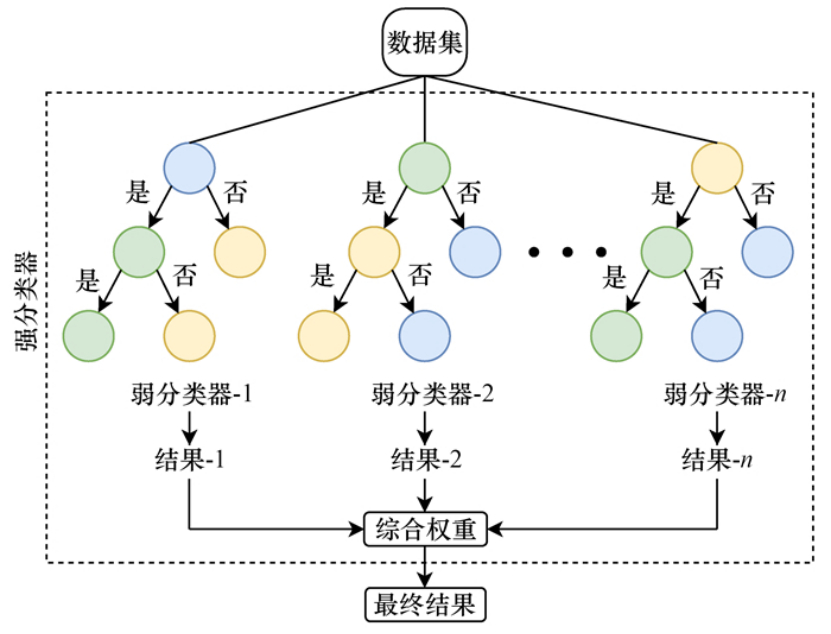
\includegraphics[width=0.7\textwidth]{figures/ensemble.png}
	\caption{集成模型的基本原理}
	\label{fig:ensemble}
\end{figure}
在选择机器学习模型时,我们主要考虑以下几个关键特性:\textbf{训练速度快、能够处理高维数据以及具备良好的泛化能力}。基于这些特性,我们选择了\textbf{XGBoost}模型。\textbf{XGBoost(Extreme Gradient Boosting)}\cite{10.1145/2939672.2939785}是一种高效且灵活的梯度提升框架,通过集成决策树模型并逐步优化,展现出卓越的性能和可扩展性,尤其在处理大规模数据集时表现优异。XGBoost的主要优点包括:
\begin{itemize}
	\item 高性能:XGBoost通过直方图优化、GPU加速以及数据/特征并行等技术,大幅提升了训练效率,相较于一般的集成模型,它能够更快速地完成训练过程。
	\item 灵活性:作为一个集成决策树模型,XGBoost不仅能够自动处理缺失值,还能处理数值型和类别型等多种类型的数据。这种灵活性使其非常契合我们数据集的特点。
	\item 准确性:XGBoost通过拟合决策树的预测残差,逐步优化树模型的结构和权重,从而提升预测准确性。这种逐步优化的方式有效地提高了模型的整体性能。
	\item 可解释性:XGBoost提供了特征重要性评估和模型解释功能,使我们能够更直观地理解模型的预测结果,以及各特征对预测结果的影响。这种可解释性对于模型的应用和改进具有重要意义。
\end{itemize}
通过这些优势,XGBoost成为我们在处理复杂数据集和追求高效、准确预测时的理想选择。
XGBoost的原理如下:
假设已经训练了$t-1$个模型,现在准备增加一个模型$f_t(x)$,使得目标函数:
\begin{equation}
	\mathcal{L}(F_{t-1}+\alpha f_t)=\sum_{i=1}^{n}l(y_i,\hat{y}^{(t)})+\Omega(f_t),
\end{equation}
最小化,其中$\hat{y}^{(t)}=F_{t-1}(x)+f_t(x)$,$\Omega(f_t)$是正则化项,$l(y_i,\hat{y}^{(t)})$是损失函数,$n$ 是样本数量。我们对损失函数$l(y_i,\hat{y}^{(t)})$在$F_{t-1}(x)+f_t(x)$处进行二阶泰勒展开,并且忽略余项,那么我们可以得到
\begin{equation}
	l(y_i,\hat{y}^{(t)})\approx\sum_{i=1}^{n}\left[l\left(y_{i},\hat{y}_{i}^{(t-1)}\right)+g_{i}f_{t}(x_{i})+\frac{1}{2}h_{i}f_{t}^{2}(x_{i})\right],
\end{equation}
其中$g_i=\nabla_{\hat{y}^{(t-1)}}l\left(y_i,\hat{y}_i^{(t-1)}\right)\quad h_i=\nabla_{\hat{y}^{(t-1)}}^2l\left(y_i,\hat{y}_i^{(t-1)}\right)$,对于每个叶子结点的预测
\begin{equation}
	f_t(x)=w_{q(x)},w\in\mathbb{R}^T,q\colon\mathbb{R}^d\mapsto\{1,2,...,T\},,,,,
\end{equation}
其中$T$是叶子结点的个数,$q(x)$是样本$x$在树中的叶子结点的索引(因为每个样本最终都会落到某个叶子节点上),$w$是叶子结点的权重,那么我们就可以定义正则化函数:
\begin{equation}
	\Omega(f_t)=\gamma T+\frac{1}{2}\lambda\sum_{i=1}^{T}w_i^2,
\end{equation}
$\gamma$和$\lambda$是超参数,分别控制叶子结点的个数和叶子结点的惩罚权重,最终的优化目标为
\begin{equation}
	\begin{aligned}
		\mathcal{L}^{(t)} & \simeq\sum_{i=1}^{n}\left[l\left(y_{i},\hat{y}_{i}^{(t-1)}\right)+g_{i}f_{t}(x_{i})+\frac{1}{2}h_{i}f_{t}^{2}(x_{i})\right]+\Omega(f_{t})
		\\
		                  & =\sum_{i=1}^{n}\left[g_{i}f_{t}(x_{i})+\frac{1}{2}h_{i}f_{t}^{2}(x_{i})\right]+\gamma T+\frac{1}{2}\lambda\sum_{j=1}^{T}w_{j}^{2}+co
		\\
		                  & =\sum_{j=1}^{T}\left[(\sum_{i\in I_{i}}g_{i})w_{j}+\frac{1}{2}(\sum_{i\in I_{i}}h_{i}+\lambda)w_{j}^{2}\right]+\gamma T+const
	\end{aligned}
\end{equation}
其中$I_j$是样本集合$\{i|q(x_i)=j\}$,也就是由于每个样本最终都会落到某个叶子结点上,因此把对样本的求和转换为对叶子结点的求和,并且$l(y_i,y^{(t-1)})$是已经确定的常数,因此最终优化目标是
\begin{equation}
	\mathcal{L}^{(t)}=\sum_{j=1}^{T}\left[(\sum_{i\in I_{i}}g_{i})w_{j}+\frac{1}{2}(\sum_{i\in I_{i}}h_{i}+\lambda)w_{j}^{2}\right]+\gamma T
\end{equation}
这是一个关于$w_i$的二次函数,可以通过求导得到最优解,令
\begin{equation}
	G_j=\sum_{i \in I_j}g_i\quad H_j=\sum_{i \in I_j}h_i,
\end{equation}
则优化目标的闭式解为
\begin{equation}
	w_{j}^{*}=-\frac{G_{j}}{H_{j}+\lambda}\quad \mathcal{L}^{(t)}=-\frac{1}{2}\sum_{i=1}^{T}\:\frac{G_{j}^{2}}{H_{j}+\lambda}+\gamma T,
\end{equation}
那么在构建决策树时,我们可以通过贪心算法,从根节点开始,对每个叶子结点,计算其最优的权重$w_j$,然后计算损失函数,
\begin{equation}
	\text{Gain}=\frac{1}{2}(\frac{G_{L}^{2}}{H_{L}+\lambda}+\frac{G_{R}^{2}}{H_{R}+\lambda}-\frac{(G_{L}+G_{R})^{2}}{H_{L}+H_{R}+\lambda})-\gamma,
\end{equation}
其中$G_L,H_L$和$G_R,H_R$分别是左右子树的梯度值,最后选择最优的划分特征和划分点,递归构建树,直到满足停止条件。
在本题中,由于是分类问题,我们使用交叉熵作为损失函数,
\begin{equation}
	l(y_i,\hat{y}_i^{(t-1)})=-\left(y_i\log(\hat{y}_i^{(t-1)})+(1-y_i)\log(1-\hat{y}_i^{(t-1)})\right)
\end{equation}
则该损失函数的梯度和二阶导数分别为
\begin{equation}
	g_i=\hat{y}_i^{(t-1)}-y_i ,\quad h_i=\hat{y}_i^{(t-1)}(1-\hat{y}_i^{(t-1)}),
\end{equation}

最终,XGBoost的算法如\autoref{alg:xgboost}所示。
\begin{algorithm}[H]
	\caption{XGBoost}
	\label{alg:xgboost}
	\begin{algorithmic}[1]
		\REQUIRE 超参数:$\lambda$ 和 $\gamma$。特征$X$,标签$Y$。停止条件:树的最大深度$K$。
		\ENSURE 集成模型XGBoost

		\STATE \textbf{计算梯度和二阶导数}:
		\FOR{每个样本 $i$}
		\STATE 计算损失函数的一阶梯度 $g_i$ 和二阶导数 $h_i$。
		\ENDFOR
		\STATE \textbf{遍历所有特征}:
		\FOR{每个特征 $j$}
		\STATE 计算所有可能的分裂点。
		\FOR{每个分裂点}
		\STATE 将数据集分为左子集 $L$ 和右子集 $R$。
		\STATE 计算左子集和右子集的梯度和二阶导数之和:
		\STATE $G_L = \sum_{i \in L} g_i, \quad H_L = \sum_{i \in L} h_i$
		\STATE $G_R = \sum_{i \in R} g_i, \quad H_R = \sum_{i \in R} h_i$
		\STATE 计算分裂增益:
		\STATE $\text{Gain} = \frac{1}{2}\left(\frac{G_L^2}{H_L + \lambda} + \frac{G_R^2}{H_R + \lambda} - \frac{(G_L + G_R)^2}{H_L + H_R + \lambda}\right) - \gamma$
		\ENDFOR
		\ENDFOR
		\STATE \textbf{选择最佳分裂点}:
		\STATE 对于每个特征,选择具有最大增益的分裂点。
		\STATE 在所有特征中,选择增益最大的分裂点作为最终的分裂点。
		\STATE \textbf{递归分裂}:
		\STATE 对于新的左子树和右子树,重复步骤2至5,直到满足停止条件
	\end{algorithmic}
\end{algorithm}
\par
对于$d$个特征,每个特征,都可以以$O(1)$的速度构建计算增益,每一层都需要$n\log n$的时间排序选出最佳特征,一共$K$层,因此整个XGBoost算法的时间复杂度为$O(Kdn\log{n})$

\vspace*{1cm}
\section{问题四}
提高由编译结果区分编译器版本的判别函数性能的建议:
\vspace*{1cm}
\subsection{自动特征提取}
特征工程将原始数据转化为更适合模型学习的特征的过程,直接影响模型的性能和准确性。然而,传统的手动特征工程存在一些缺陷。首先,手动特征工程依赖于领域专家的知识和经验,这将导致特征选择的主观性和局限性。其次,手动提取特征通常是一个耗时且繁琐的过程,尤其在高维数据或复杂数据结构的情况下,难以保证全面和高效。因此,如果要提高模型的区分度和性能,我们可以考虑采用深度学习技术来进行自动特征提取我们构想了一个基于协同注意力机制的模型。具体来说,首先将源文件和对应的汇编文件转换为词向量嵌入表示。然后,利用基于 Transformer 的自注意力机制来捕捉文件内部的语义特征。为了更好地理解源文件与汇编文件之间的关系,进一步采用 Cross-Attention 机制来提取它们之间的语义相似性和结构相异性。这种方法的优势在于,它能够自动捕捉不同编译器版本之间在语义和结构上的细微差异,这些差异可以作为有效的特征,用于构建高效的分类模型。
\vspace{1cm}
\subsection{增加数据集多样性}
考虑到不同领域的源代码会存在很大的差异,例如同为C++程序代码,后端服务器代码往往倾向于网络和IO操作,而游戏的代码则会包含到大量的图形渲染和物理计算,因此不同领域的源代码在同一个版本的编译器编译的编译结果存在很大差异。此外,即使是同一个领域的源代码,不同规模的源代码之间也会存在非编译器造成的差异。最后编译器版本之间的差距主要是体现在对于不同版本的语言支持以及静态代码优化技术,而后者一般要通过编译指令开启代码优化才能体现。鉴于以上分析,我们可以通过以下几种方式来增加数据集的多样性,提高模型的泛化能力:
\begin{itemize}
    \item 不同类型的程序:收集多种类型的程序(如计算密集型、IO 密集型、混合型)进
    行编译,提取汇编结果。
    \item 不同规模的程序:从小规模到大规模的程序进行编译,确保模型能泛化到不同复
    杂度的代码。
    \item 编译优化级别:使用不同的优化级别(如-O0,-O1,-O2,-O3)进行编译,捕捉
    编译器在不同优化下的行为差异。
\end{itemize}
\vspace*{1cm}
\subsection{结合静态和动态特征}
除了源代码和汇编代码之外,我们还可以考虑结合静态特征和动态特征来提高模型的区分度。具体来说,我们可以提取以下两类特征:
\begin{itemize}
    \item 静态特征:提取静态汇编特征,如指令频率、寄存器使用率、基本块大小。
    \item 动态特征:运行程序,收集运行时的行为特征,如执行路径、内存访问模式、CPU
    使用率。
 我们可以通过结合静态和动态的特征进行分析,更全面地了解编译器版本之间的差异,提高模型的泛化能力。
\end{itemize}

\vspace*{1cm}
\section{总结与展望}
编译器版本识别在现实中具有重要的应用价值。通过精确识别编译器的版本,能够帮助检测和预防与编译器相关的安全漏洞。例如,不同版本的编译器在处理某些指令集时可能存在特定的安全隐患,及时识别这些版本有助于安全团队采取针对性的防护措施,从而提升软件系统的整体安全性。

本文提出了一种基于操作码频率、寄存器使用率以及Bigram数量等特征的提取方法,用于区分和识别不同版本的编译器。通过对汇编代码的特征提取,能够捕捉到编译器版本之间的细微差异,使得模型在版本识别方面的准确性得到了显著提升。这种方法不仅为编译器版本的识别提供了新的技术路径,也为提高软件安全性提供了有力支持。该方法的应用可以扩展到各种编译器相关的安全分析场景,为开发和安全团队在应对复杂的安全威胁时提供了更加精细化的工具和手段。
\vspace*{1cm}

%%----------- 参考文献 -------------------%%
%在reference.bib文件中填写参考文献,此处自动生成
\newpage
\reference
\newpage
\appendix

\section*{关键程序代码}
\vspace*{1cm}
\subsection*{汇编文件预处理}
\begin{lstlisting}
import os
import re

def process_assembly_file(input_file, output_file):
    # 读取原始汇编文件
    with open(input_file, 'r', encoding='utf-8') as file:
        lines = file.readlines()

    # 创建一个新的列表来存储修改后的内容
    processed_lines = []

    # 遍历原文件的每一行
    for line in lines:
        # 将逗号替换为空格
        line = line.replace(',', ' ')

        # 去除每行的前后空格
        stripped_line = line.strip()

        # 跳过以 . 开头或以 : 结尾的行
        if stripped_line.startswith('.') or stripped_line.endswith(':'):
            continue

        # 按空格分割行内的内容,得到每个单词
        words = re.split(r'\s+', stripped_line)

        # 处理每个单词
        processed_words = []
        for word in words:
            # 查找是否有括号,并替换为括号内的内容
            match = re.search(r'\((%[a-zA-Z0-9]+)\)', word)
            if match:
                word = match.group(1)

            # 处理以 $ 开头的单词
            if word.startswith('$'):
                if re.match(r'\$\d+', word):  # 如果 $ 后跟数字
                    word = '$0'
                elif re.match(r'\$-', word):  # 如果 $ 后跟负号
                    word = '$0'
                elif word.startswith('$.'):  # 如果 $ 后跟 .
                    word = '$.'
                elif word.startswith('$g'):  # 如果 $ 后跟 g
                    word = '$g'

            processed_words.append(word)

        # 将处理后的单词重新组合成一行
        processed_line = ' '.join(processed_words)
        processed_lines.append(processed_line + '\n')  # 保持行的格式

    # 写入新的汇编文件
    with open(output_file, 'w', encoding='utf-8') as file:
        file.writelines(processed_lines)


def process_all_files(input_folder, output_folder):
    # 如果输出文件夹不存在,则创建
    if not os.path.exists(output_folder):
        os.makedirs(output_folder)

    # 遍历输入文件夹中的所有文件
    for filename in os.listdir(input_folder):
        # 构造完整的文件路径
        input_file = os.path.join(input_folder, filename)
        output_file = os.path.join(output_folder, filename)

        # 处理每个文件
        process_assembly_file(input_file, output_file)


input_folders = ['8.4.0', '10.2.0', '11.3.0', '12.2.0', '13.2.0']
output_folders = [f"{folder}_processed" for folder in input_folders]

print(output_folders)

# 处理所有文件
for input_folder, output_folder in zip(input_folders, output_folders):
    process_all_files(input_folder, output_folder)

print("所有文件处理完毕。")

\end{lstlisting}
\vspace*{1cm}
\subsection*{特征提取}

\begin{lstlisting}
import csv
import os
from collections import Counter

file_count = 0  # 初始化文件计数器


def process_folder(folder_name):
    data = []
    global file_count
    file_count += 1  # 每处理一个文件夹,计数器加一
    for filename in os.listdir(folder_name):
        print(f"Processing {filename}...")
        if 'test' not in filename:
            print(f"Skipping {filename}...")
            continue
        file_path = os.path.join(folder_name, filename)
        with open(file_path, 'r') as file:
            word_counter = Counter()
            bigram_counter = Counter()
            first_word_list = []

            for line in file:
                words = line.strip().split()
                if not words:
                    continue
                first_word_list.append(words[0])
                word_counter.update(words)
                bigram_counter.update(zip(words[:-1], words[1:]))

            # 计算四元组(四个连续单词)的频率
            quadgram_counter = Counter(
                zip(first_word_list[:-3], first_word_list[1:-2],
                    first_word_list[2:-1], first_word_list[3:]))

            # 筛选频率大于10的特征
            word_features = {
                word: count
                for word, count in word_counter.items() if count > 10
            }
            bigram_features = {
                " ".join(bigram): count
                for bigram, count in bigram_counter.items() if count > 10
            }
            quadgram_features = {
                " ".join(quadgram): count
                for quadgram, count in quadgram_counter.items() if count > 10
            }

            # 构建一行数据
            features = {
                **word_features,
                **bigram_features,
                **quadgram_features
            }
            features['label'] = file_count  # 标签为当前文件的编号

            data.append(features)

    return data


def save_to_csv(data, output_file):
    keys = set()
    for row in data:
        keys.update(row.keys())

    keys = sorted(keys)  # 按字母排序,确保一致性
    with open(output_file, 'w', newline='') as csvfile:
        writer = csv.DictWriter(csvfile, fieldnames=keys)
        writer.writeheader()
        for row in data:
            writer.writerow(row)


# 定义已处理的文件夹列表
processed_folders = [
    '8.4.0_processed', '10.2.0_processed', '11.3.0_processed',
    '12.2.0_processed', '13.2.0_processed'
]

# 初始化用于保存所有文件夹数据的列表
all_data = []

# 遍历每个文件夹并处理数据
for folder in processed_folders:
    folder_data = process_folder(folder)
    all_data.extend(folder_data)

# 保存合并后的数据到CSV文件
save_to_csv(all_data, 'no_our_data.csv')

\end{lstlisting}
\vspace*{1cm}
\subsection*{模型建立}
\begin{lstlisting}
import pandas as pd
from sklearn.model_selection import train_test_split
import lightgbm as lgb
from sklearn.metrics import confusion_matrix, classification_report, ConfusionMatrixDisplay
import matplotlib.pyplot as plt
from sklearn.manifold import TSNE

df = pd.read_csv('processed_data2.csv')
df.fillna(0, inplace=True)
df[f'testb %al'], df['label'] = df['testb %al'], df['label']
X = df.drop(columns=['label'])
y = df['label']
y = y - 1

num_others_data = 1002
file1_idx = [i + num_others_data * j for i in range(1) for j in range(5)]
file2_idx = [i + num_others_data * j for i in range(1, 2) for j in range(5)]
our_data_idx = [i + num_others_data * j for i in range(2) for j in range(5)]
others_data_idx = df.index.difference(our_data_idx + file1_idx + file2_idx)
file1_data = X.iloc[file1_idx]
file2_data = X.iloc[file2_idx]
our_data = X.iloc[our_data_idx]

tsne = TSNE(n_components=2, perplexity=2, random_state=42, n_jobs=-1)
X_tsne = tsne.fit_transform(X)
df_tsne = pd.DataFrame(X_tsne, columns=['Component 1', 'Component 2'])
df_tsne['label'] = y
# 绘制 t-SNE 图像,使用标签 y 进行着色
plt.figure(figsize=(10, 10))
s = 30
scatter = plt.scatter(df_tsne['Component 1'],
                      df_tsne['Component 2'],
                      c=df_tsne['label'],
                      cmap='tab10',
                      marker='o',
                      edgecolor='k',
                      s=s)
plt.scatter(df_tsne.loc[file1_idx]['Component 1'],
            df_tsne.loc[file1_idx]['Component 2'],
            c='fuchsia',
            marker='o',
            edgecolor='k',
            label='file1',
            s=s)
plt.scatter(df_tsne.loc[file2_idx]['Component 1'],
            df_tsne.loc[file2_idx]['Component 2'],
            c='lightpink',
            marker='o',
            label='file2',
            edgecolor='k',
            s=s)

legend1 = plt.legend(*scatter.legend_elements(),
                     title="Labels",
                     loc='upper left')
plt.gca().add_artist(legend1)
plt.legend(loc='upper right')
plt.title('t-SNE Visualization')
plt.grid(True)
plt.show()

from xgboost import XGBClassifier
import warnings
from sklearn.model_selection import train_test_split

X_train, X_test, y_train, y_test = train_test_split(
    X,
    y,
    test_size=0.2,
)
warnings.filterwarnings('ignore')
xgb_params = {
    "objective": "binary:logistic",  # 目标函数:二分类逻辑回归
    "max_depth": 50,  # 树的最大深度
    "eta": 0.4,  # 学习率
    "subsample": 1,  # 采样率
    'sampling_method': 'uniform',  # 采样算法,uniform:均匀采样,gradient_based:梯度采样
    "colsample_bytree": 1,  # 构建每棵树时,使用特征的比例
    "colsample_bylevel": 1,  # 树的每一级的每一次分裂,对特征的采样比例
    "reg_lambda": 1,  # L2 正则化
    "reg_alpha": 1,  # L1 正则化
    "min_child_weight": 1,  # 最小的叶子节点样本权重和
    "gamma": 0,  # 节点分裂所需的最小损失函数减少量
    "eval_metric": "logloss",  # 评估指标:对数损失
    "scale_pos_weight": 1,  # 用于处理类别不平衡 negative:positive
    "tree_method": "hist",  # 树构建算法 ['exact', 'approx', 'hist', 'gpu_hist']
    'device': 'gpu',
    "nthread": -1,  # 使用所有可用线程
    # "seed":42,  # 随机数种子
    "n_estimators": 100,  # 决策树个数
    "booster": "gbtree",  # 基本模型
    'max_delta_step': 0,  # 限制每棵树权重改变的最大步长,0表示没有约束
}
model = XGBClassifier(**xgb_params)
model.fit(X_train, y_train)

y_pred = model.predict(X)
y_pred_ours = y_pred[file2_idx]
cm = confusion_matrix(y[file2_idx], y_pred_ours)
disp = ConfusionMatrixDisplay(confusion_matrix=cm)
disp.plot(cmap="Blues")
plt.title('Confusion Matrix')

y_pred = model.predict(X_test)
print(classification_report(y_test, y_pred))

\end{lstlisting}

\end{document}